% Settings for the default beamer theme
\documentclass[english, aspectratio=169]{beamer}
\usepackage[T1]{fontenc}
\usepackage[utf8]{inputenc}
\usepackage{tabularx}
\usepackage{babel}
\usepackage[ruled,vlined]{algorithm2e}
\SetAlgorithmName{Algoritmus}{algoritmus}{List of Algorithms}
\setcounter{secnumdepth}{3}
\setcounter{tocdepth}{3}

\makeatletter

\newcommand\makebeamertitle{\frame{\maketitle}}

% (ERT) argument for the TOC
\AtBeginDocument{%
  \let\origtableofcontents=\tableofcontents
  \def\tableofcontents{\@ifnextchar[{\origtableofcontents}{\gobbletableofcontents}}
  \def\gobbletableofcontents#1{\origtableofcontents}
}

% Theme settings
\usetheme{Frankfurt}
\usecolortheme{default}
\usefonttheme[onlymath]{serif}

% Template settings
\setbeamertemplate{navigation symbols}{}
\setbeamertemplate{blocks}[rounded][shadow=false]
\setbeamertemplate{title page}[default][colsep=-4bp, rounded=true, shadow=false]
\makeatother

% Define a custom darker red color
\definecolor{DarkerRed}{RGB}{139,0,0} % Adjust the RGB values as needed

% Use the newly defined color in Beamer theme elements
\setbeamercolor{structure}{fg=DarkerRed} % Changes basic structural elements to Darker Red
\setbeamercolor{title in head/foot}{bg=DarkerRed} % Changes the title in header/footer to Darker Red


\begin{document}

% Title page
\section{Bevezetés}
\title[]{Üzleti Elemzések Módszertana}
\subtitle{5. Előadás: Együttes tanulás}
\author[Kuknyó Dániel]{Kuknyó Dániel\\Budapesti Gazdasági Egyetem}
\date{2023/24\\2.félév}
\makebeamertitle

% Table of contents slide
\begin{frame}
\tableofcontents{}
\end{frame}

% Table of contents of the current section
\begin{frame}
\tableofcontents[currentsection]
\end{frame}

\begin{frame}{Az együttes tanulás mögötti intuíció}
\begin{columns}
\begin{column}{.5\textwidth}
\begin{itemize}
	\item Egy gazda szeretné lemérni, milyen a hőmérséklet a szőlős birtokán. 
	\item A birtok egy hegyoldalban fekszik, ezért a szőlőtőkéket eltérő időjárási hatások érik.
\end{itemize}
\end{column}
\begin{column}{.5\textwidth}
\begin{center}
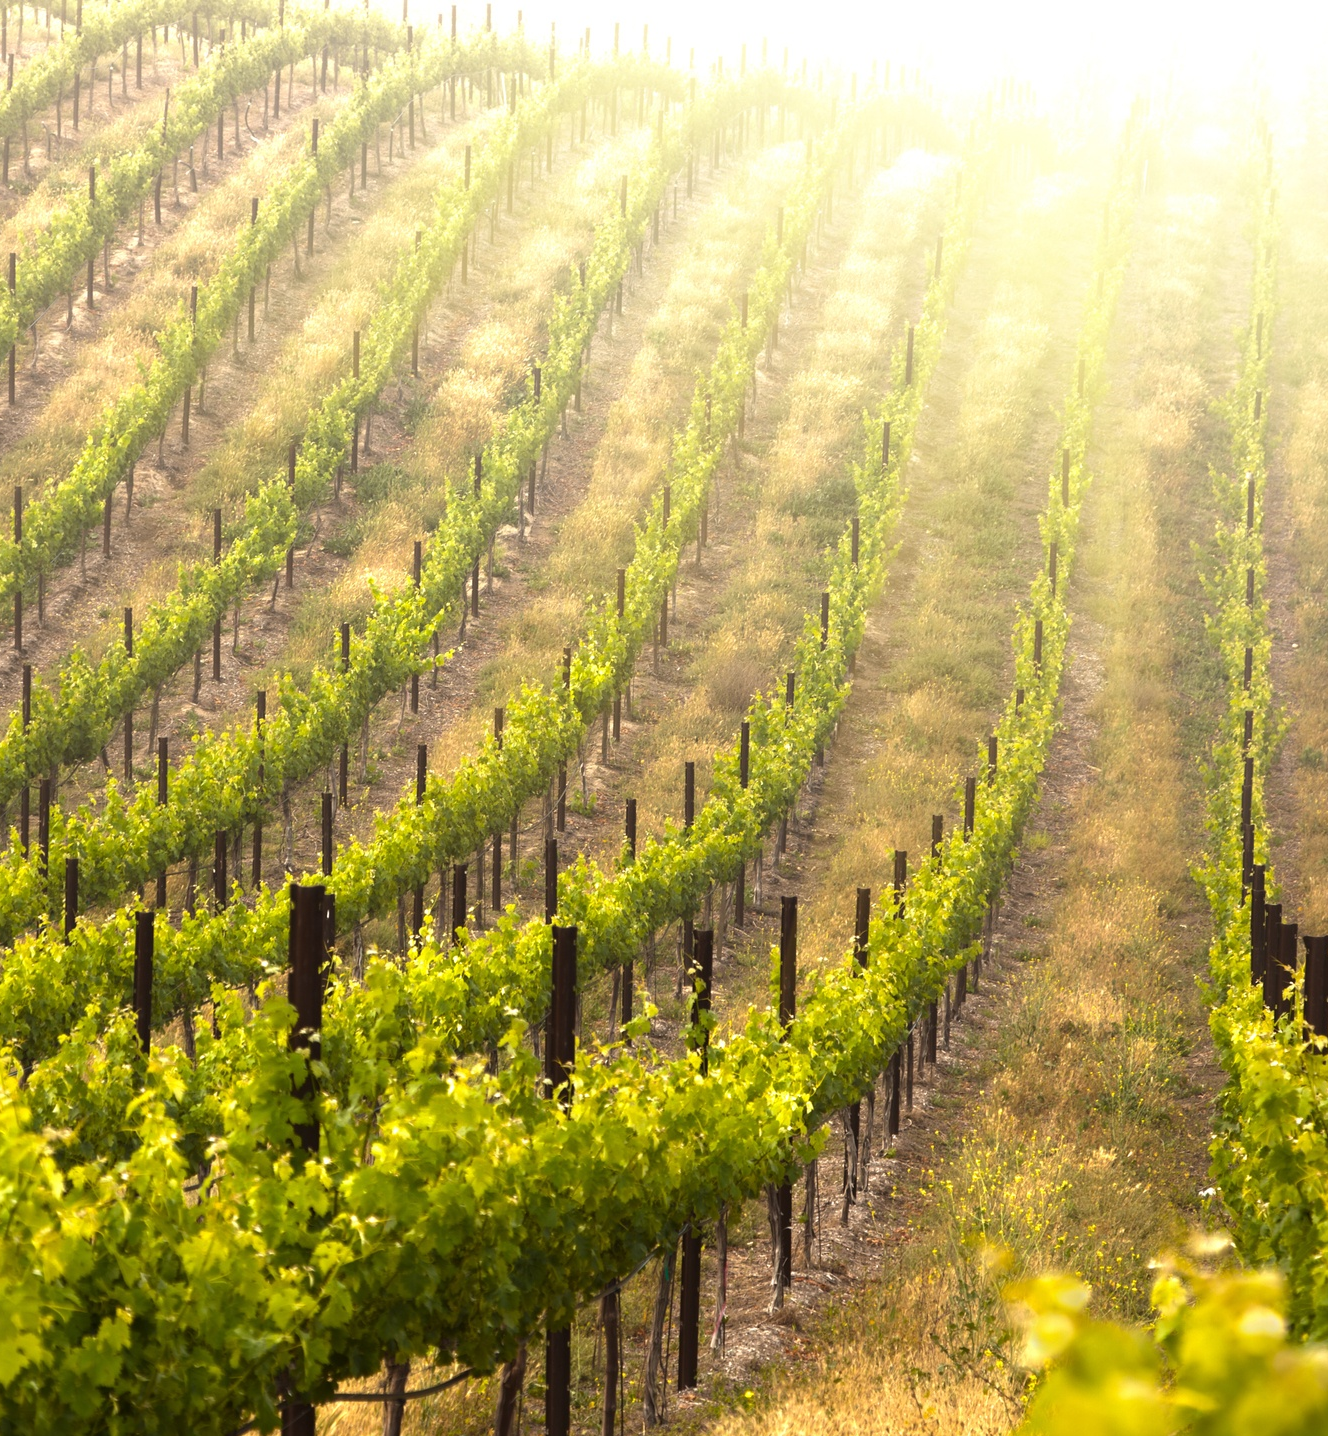
\includegraphics[width=7cm, height=5cm, keepaspectratio]{images/ensemble_2.png}
\end{center}
\end{column}
\end{columns}
\end{frame}

\begin{frame}{Példa: szavazó osztályozók}
\begin{columns}
\begin{column}{.5\textwidth}
A következő példában 10 osztályozó modell feladata, hogy megbecsüljék, melyik oldalára fog esni egy torzított pénzérme.\par\medskip
A pénzérme 51\% valószínűséggel esik fejre, 49\% eséllyel pedig írásra.\par\medskip
1000 dobás után 75\%, hogy a modellek valószínűsége fejt fog szavazni. Ugyanez a valószínűség 10000 dobás után 97\%.\par\medskip
A szavazó osztályozók nagyobb pontosságot érnek el együttesen, mint a modellcsoport bármelyik tagja. 
\end{column}
\begin{column}{.5\textwidth}
\begin{center}
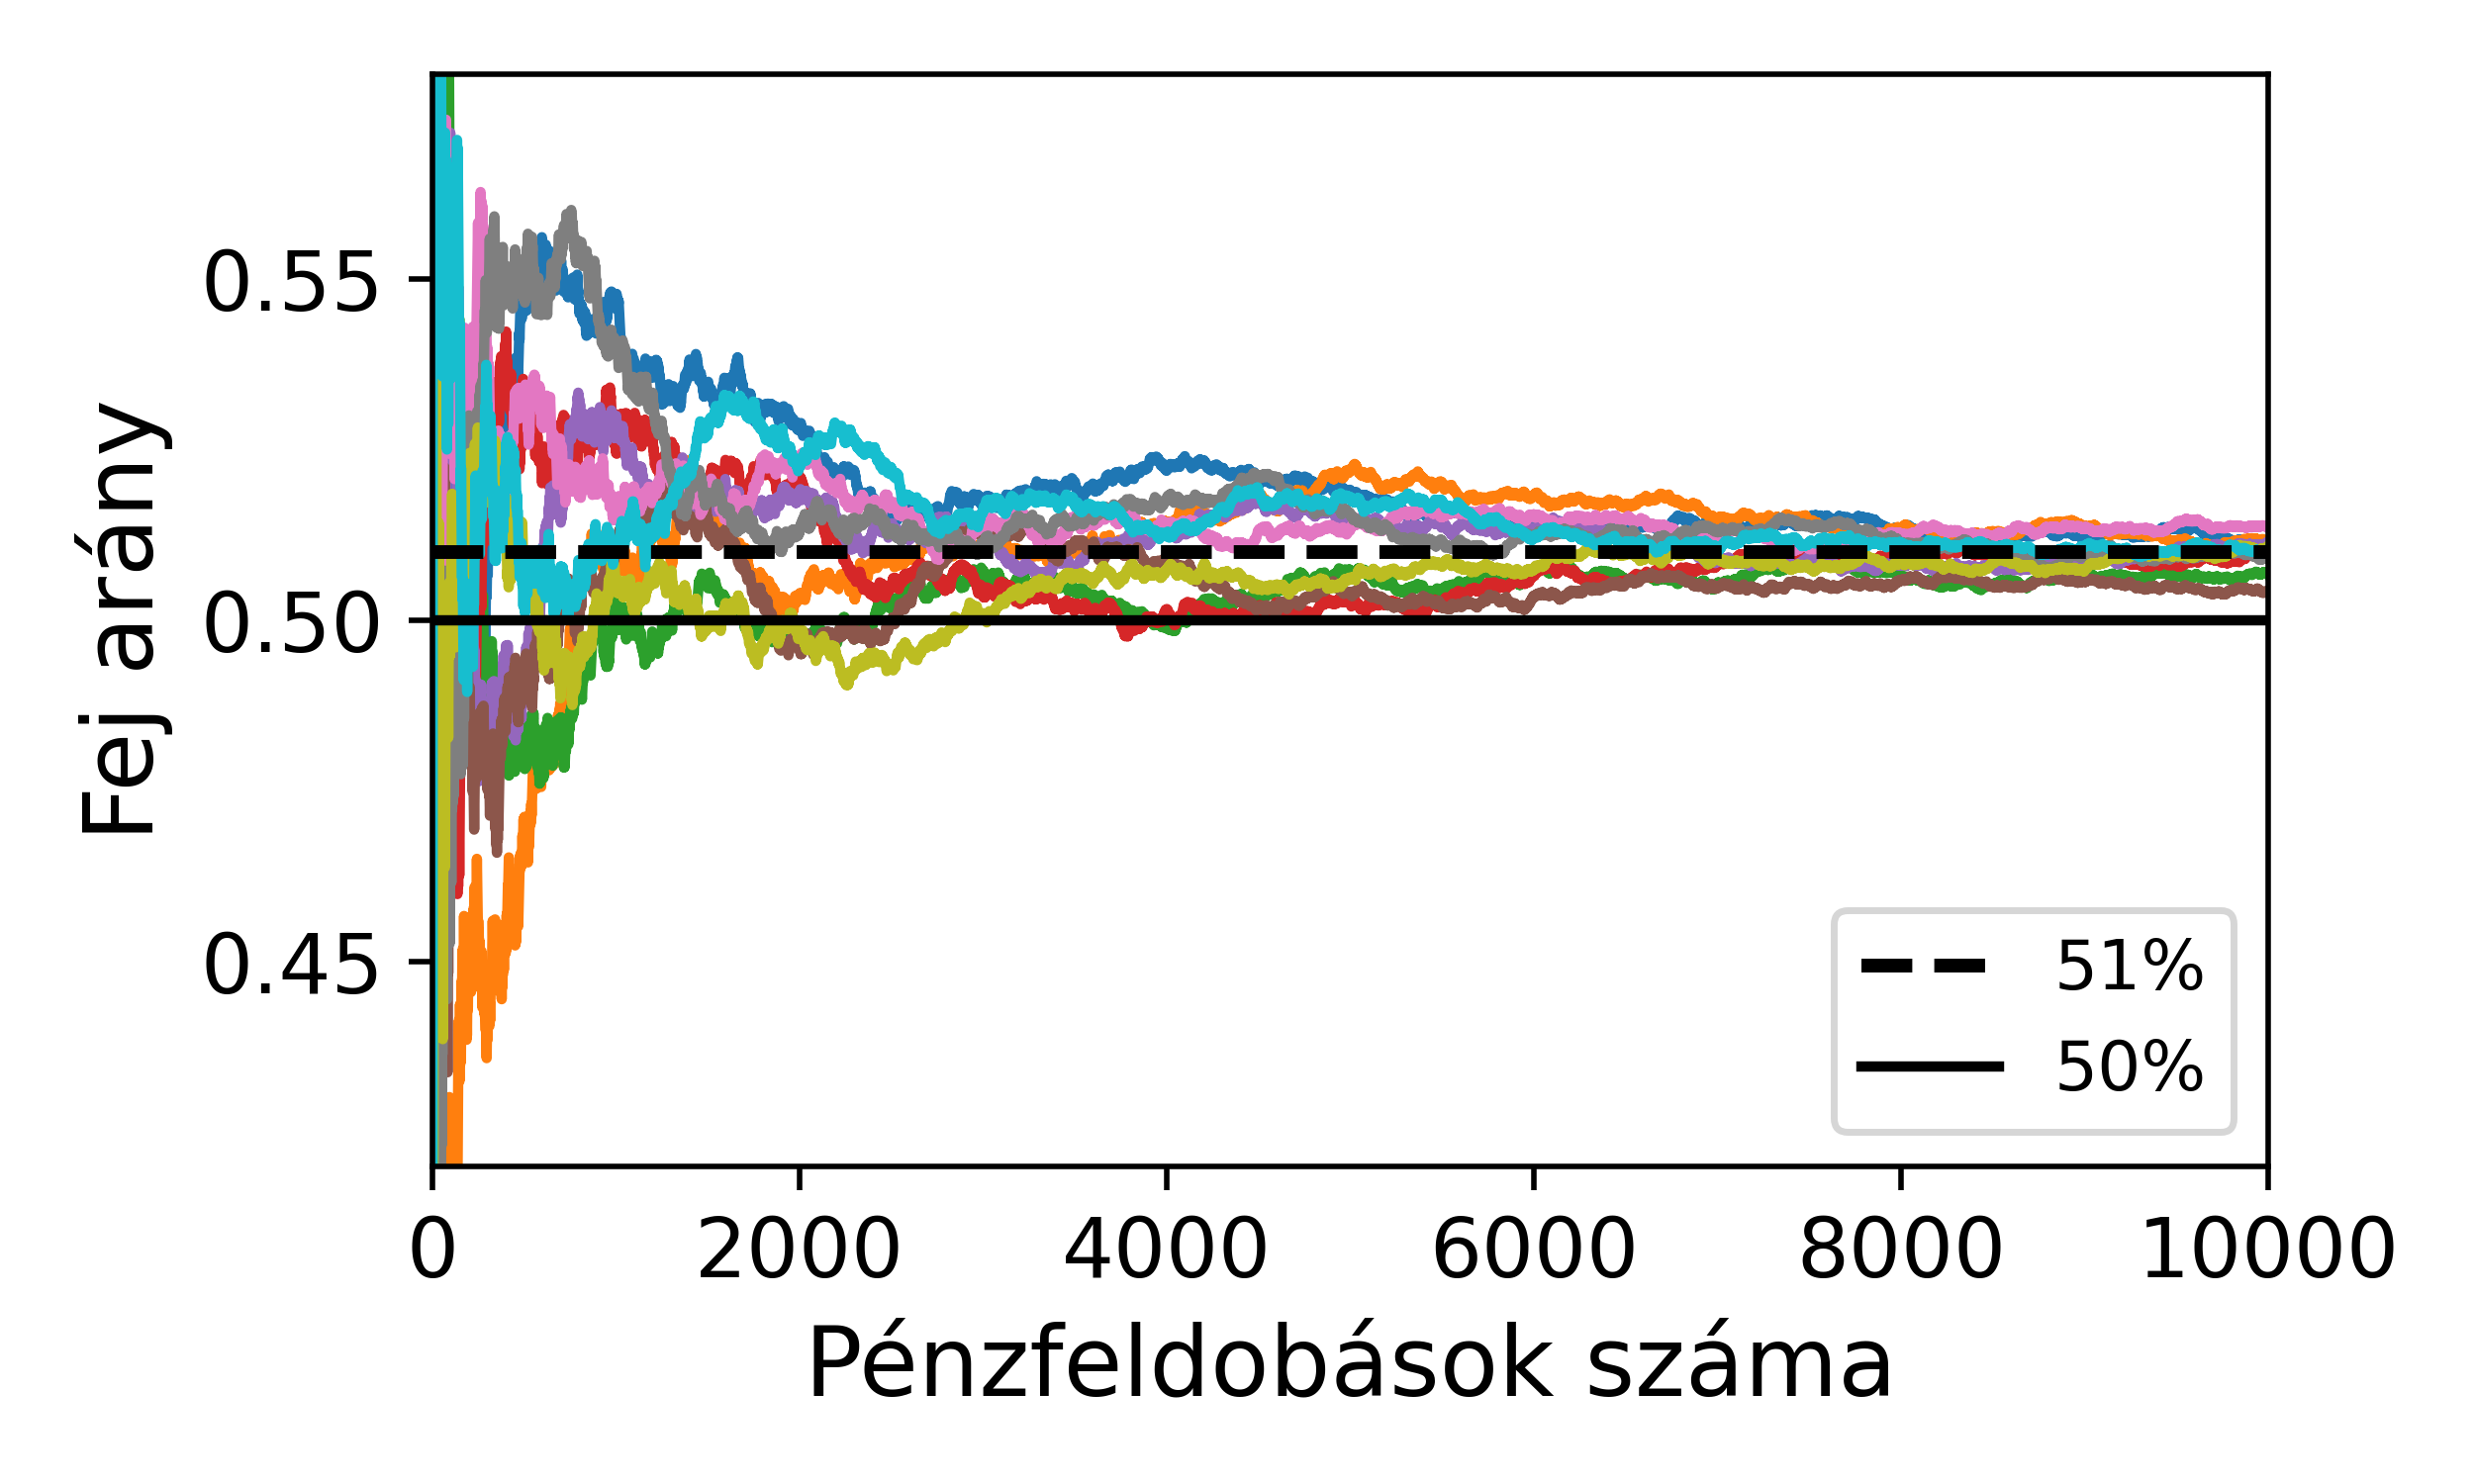
\includegraphics[width=7cm, height=7cm, keepaspectratio]{images/ensemble_1.png}
\end{center}
\end{column}
\end{columns}
\end{frame}

\begin{frame}{Szavazó osztályozók}
\begin{columns}
\begin{column}{.5\textwidth}
A szavazó osztályozó kifejezés modellek egy csoportjára utal, amelyben a modellek \textbf{egymástól függetlenül képesek predikciót adni} egy adott mintaegyedre vonatkozóan.\par\smallskip
A szavazó osztályozó a végső predikciót úgy állítja elő, hogy \textbf{a benne lévő modellek predikcióit aggregálja} valamilyen módszertan szerint pl. kiválasztja belőle a leggyakoribb elemet. 
\end{column}
\begin{column}{.5\textwidth}
\begin{center}
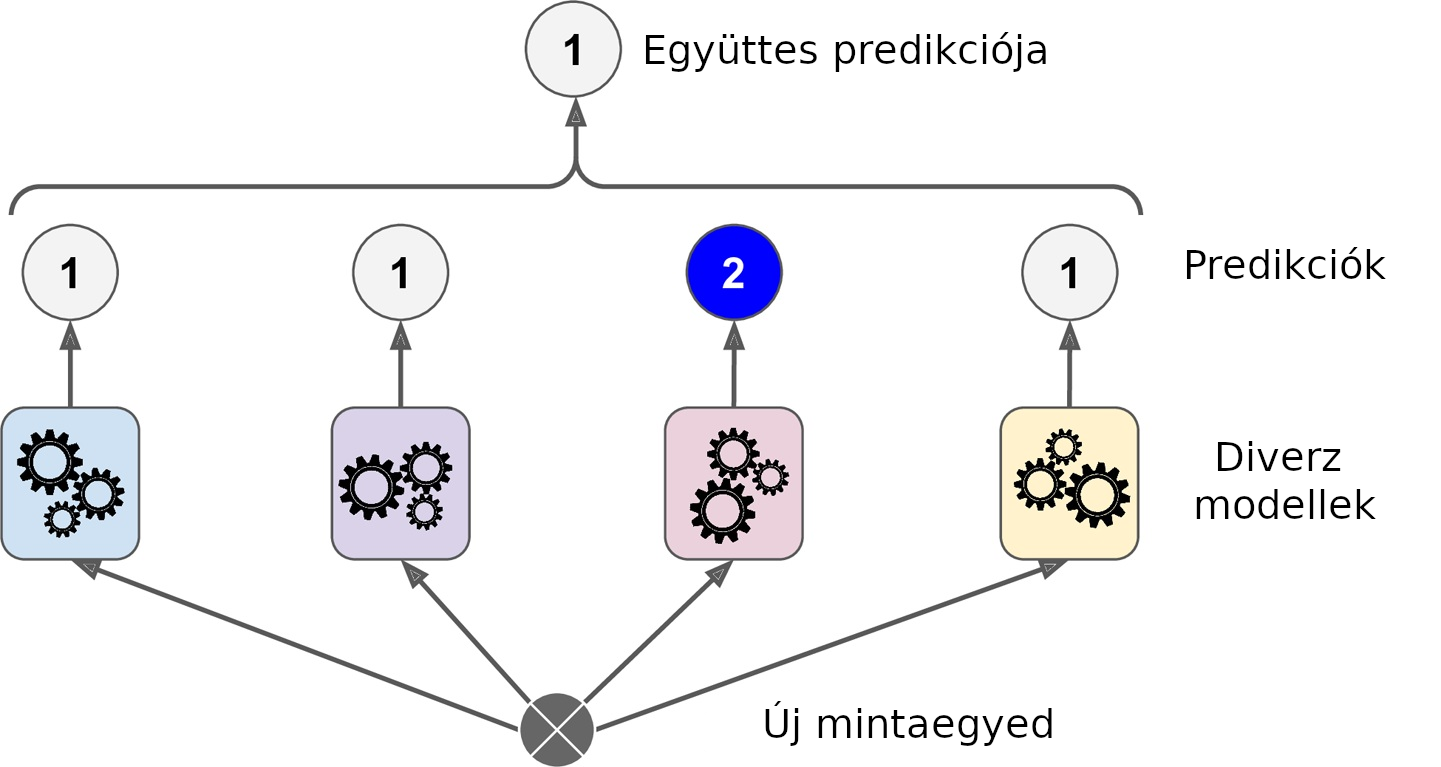
\includegraphics[width=7cm, height=7cm, keepaspectratio]{images/ensemble_3.png}
\end{center}
\end{column}
\end{columns}
\end{frame}

\begin{frame}{Bagging és Pasting}
\begin{columns}
\begin{column}{.5\textwidth}
Az együttes tanuló modellek taníthatók az adathalmaz különböző részhalmazain. Ez robusztusabb modellt fog eredményezni, ami jobb általánosító képességeket jelent éles felhasználásban.
\only<1>{\begin{block}{Bagging}
Együttes tanulási módszer, melyben a modellek \textbf{visszatevés nélküli mintavétellel} kapják meg a saját tanító mintájukat.
\end{block}} 
\only<2>{\begin{block}{Pasting}
Együttes tanulási módszer, melyben a modellek \textbf{visszatevéses mintavétellel} kapják meg a saját tanító mintájukat.
\end{block}}
\end{column}
\begin{column}{.5\textwidth}
\begin{center}
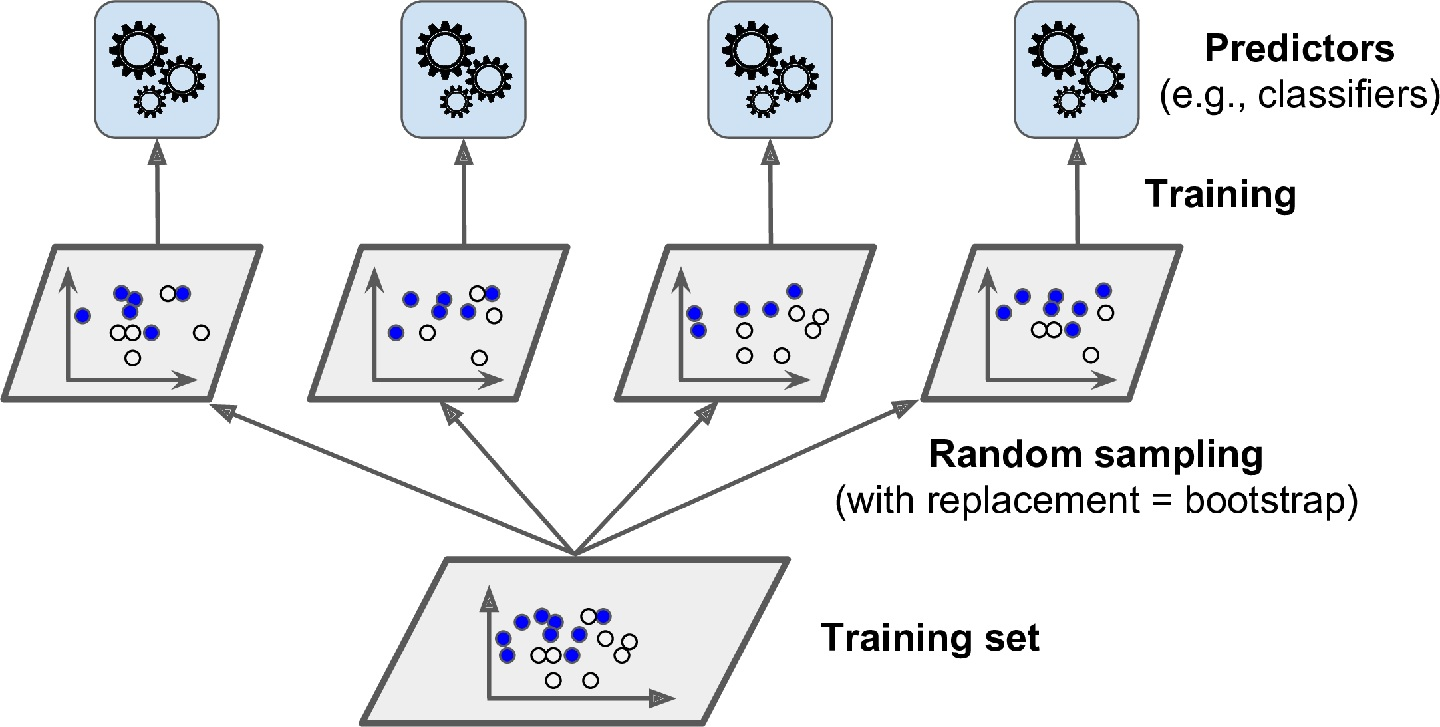
\includegraphics[width=7cm, height=7cm, keepaspectratio]{images/ensemble_4.png}
\end{center}
\end{column}
\end{columns}
\end{frame}

\section{AdaBoost}

\begin{frame}
\tableofcontents[currentsection]
\end{frame}

\begin{frame}{AdaBoost: 1}
\begin{columns}
\begin{column}{.5\textwidth}
\begin{block}{AdaBoost}
Az együttes tanulás súlyozott változata. A modellek szekvenciálisan állnak elő olyan módon, hogy az új modell mindig tanul az elődje hibájából. 
\end{block}
\begin{enumerate}
	\item Az algoritmus minden mintaegyedhez $\frac{1}{n}$ kezdeti súlyt rendel, ahol $n$ az összes a minta halmaz mérete.
\end{enumerate}
\end{column}
\begin{column}{.5\textwidth}
\begin{center}
\begin{tabular}{|c|c|c|c|c|}
\hline
$x_1$ & $x_2$ & $x_3$ & $y$ & $w$\\
\hline
 & & & & $\frac{1}{n}$ \\
\hline
 & & & & $\frac{1}{n}$ \\
\hline
 & & & & $\frac{1}{n}$ \\
\hline
\end{tabular}
\end{center}
\end{column}
\end{columns}
\end{frame}

\end{document}

























